\chapter{\label{c:speedmeter-intro}The \SSMEXPT{}: introduction and technical design}
\chaptermark{\SSM{} introduction and technical design}

This chapter introduces the ongoing \SSMEXPT{} in Glasgow and serves as background for the work presented in Chapters \ref{c:speedmeter-control} and \ref{c:esd-concept}. The first half of this chapter discusses the measurement of test mass displacement and speed in the context of interferometers, and compares the sensitivity of the two measurements. The second half details the particular setup employed in the Glasgow experiment.

\section{\label{sec:pos-speed-meters}Position and \SM{}s}

\subsection{\label{sec:position-meter-measurement}Sensitivity of a position meter}
In an ordinary \FPMI{} the motion of each cavity in the longitudinal direction either increases or decreases the round-trip phase of the light in that arm. The phase difference of the two recombined beams at the beam splitter then leads to a signal at the output port proportional to the differential phase which can be measured using a heterodyne or homodyne readout as discussed in Section\,\ref{sec:readout}.

The presence of classical light power in the arms leads to \gls{DC} radiation pressure which imparts a force upon the test masses. The reaction of the mirrors' restoring force, either from its pendulum in a suspended experiment or its mount on a table-top experiment, means that the interferometer can be held at the operating point as discussed in Section\,\ref{sec:operating-point} by making microscopic corrections to the position of the optic. The output signal can be calculated by considering \emph{input-output relations} which define the effect that input light has at the output given the interferometer dynamics.

\subsubsection{Input-output relations}
We use the \emph{two-photon formalism} \cite{Caves1985, Schumaker1985} in order to calculate the effect that the interferometer has on the light's amplitude and phase. This represents the input and output in terms of its \emph{cosine} and \emph{sine} quadratures, namely:
\begin{align}
  \vec{a} &=
  \begin{pmatrix}
    a_c \\
    a_s
  \end{pmatrix} \\
  \vec{b} &=
  \begin{pmatrix}
    b_c \\
    b_s
  \end{pmatrix},
\end{align}
where $\vec{a}$ is the input field and $\vec{b}$ is the output field. The output for an interferometer can be expressed as the sum of the signal from the input scaled by the interferometer dynamics and the noise present at the detector \cite{Danilishin2015}:
\begin{equation}
  \label{eq:ifo-output-signal}
  \vec{b} = \vec{R} \frac{h}{h_{\text{SQL}}} + \mathbb{T} \vec{a},
\end{equation}
where $\vec{R}$ is the response of the interferometer from unit mirror motion to the output, $\frac{h}{h_{\text{SQL}}}$ is the motion of the mirrors in terms of strain normalised to the \gls{SQL} as discussed in Section\,\ref{sec:sql} and $\mathbb{T}$ represents the transfer matrix of the input fields to the output fields.

The differential arm response, $\vec{R}_{\left( - \right)}$, is given by:
\begin{equation}
  \label{eq:fp-mich-response}
  \vec{R}_{\left( - \right)} = \text{e}^{\text{i} \beta_{\text{FP}}} \sqrt{2 \kappa} \vec{H},
\end{equation}
where $\beta_{\text{FP}}$ is the round-trip phase of the light in the arms, $\kappa$ is the optomechanical coupling factor (as introduced in Section\,\ref{sec:sql}) and $\vec{H}$ represents the readout angle or \emph{quadrature}, $\zeta$. The round-trip phase is defined:
\begin{equation}
  \beta_{\text{FP}} = \arctan{\frac{f}{\gamma_{\text{arm}}}},
\end{equation}
where $f$ is frequency and $\gamma_{\text{arm}}$ is the \FP{} cavity half-bandwidth (see Appendix\,\ref{sec:cavity-fom}). $\vec{H}$ is defined as the cosine and sine quadratures of the readout angle:
\begin{equation}
  \vec{H} =
  \begin{pmatrix}
    \cos \zeta \\
    \sin \zeta
  \end{pmatrix}.
\end{equation}
The effect that the mirror dynamics have on the readout is governed by $\kappa_{\text{MI}}$ defined for a \MI{} in Equation\,\ref{eq:optomechanicalcoupling}. This models the effect that a force applied to a mirror has on its position. Mirrors suspended from pendulum systems can be approximated at high frequencies to be free masses, where the effect an applied force has on the position is diminished at higher frequencies, and in the case of a \FPMI{} this force-to-displacement filtering effect scales as $\frac{1}{f^2}$ below the cavity's pole frequency, and $\frac{1}{f^4}$ above it.

The term $\mathbb{T}$ can be further broken down:
\begin{equation}
  \mathbb{T} = \text{e}^{2 \text{i} \beta_{\text{FP}}}
  \begin{pmatrix}
    1 & 0 \\
    -\kappa & 1
  \end{pmatrix},
\end{equation}
showing that the optomechanical coupling factor transforms the input $\vec{a}$ in the cosine (amplitude) quadrature into the sine (phase) quadrature governed by the mirror dynamics on its way to the output. The matrix of noise power spectral densities for the quadratures of the light at the output port, $\mathbb{S}$, is given by averaging over all frequencies:
\begin{equation}
  \mathbb{S} = \left< \vec{b} \cdot \vec{b}^{\dag} \right>,
\end{equation}
Expanding the terms we get:
\begin{equation}
  \mathbb{S} =
  \begin{pmatrix}
    1 & 0 \\
    -\kappa & 1
  \end{pmatrix}
  \left< \vec{a} \cdot \vec{a}^{\dag} \right>
  \begin{pmatrix}
    1 & -\kappa \\
    0 & 1
  \end{pmatrix},
\end{equation}
where $h$ in Equation\,\ref{eq:ifo-output-signal} has been set to \num{0} to remove signal.

\subsubsection{Sensitivity of a \FPMI{}}
In the case of \gls{DC} readout as discussed in Section\,\ref{sec:homodyne-readout} and used in current generation detectors, the readout angle $\zeta = \SI{90}{\degree}$ represents the phase quadrature:
\begin{equation}
  \vec{H}_{\text{dc}} =
  \begin{pmatrix}
    0 \\
    1
  \end{pmatrix}.
\end{equation}

We can calculate the signal at the \gls{DC} readout of the \FPMI{}, $O_{\text{dc}}$, as a function of differential arm cavity motion $h_{\left( - \right)}$ by rearranging Equation\,\ref{eq:ifo-output-signal}:
\begin{equation}
  \frac{O_{\text{dc}}}{h_{\left( - \right)}} = \frac{\text{e}^{\text{i} \beta_{\text{FP}}} \sqrt{2 \kappa_{\text{MI}}}}{h_{\text{SQL}}}.
\end{equation}
This is shown in Figure\,\ref{fig:fp-mich-response} for arm length \SI{1}{\kilo\meter}, mirror mass \SI{40}{\kilo\gram}, laser wavelength \SI{1064}{\nano\meter} and cavity half-bandwidth \SI{250}{\hertz}.

\begin{figure}
  \centering
  \includegraphics[width=\columnwidth]{graphics/generated/from-python/40-fp-mich-response.pdf}
  \caption[Response of a \FPMI{} to differential arm cavity motion]{\label{fig:fp-mich-response}Response of a \FPMI{} to differential arm cavity motion. This shows the signal that would appear at a photodetector placed at the output of the interferometer given unit differential motion of the cavity. The cavity provides a signal with the same response for motion at frequencies below the cavity's pole frequency. Beyond the pole, the response is reduced as the motion becomes faster than the cavity's storage time.}
\end{figure}

Normal, unsqueezed vacuum noise at the input has equal noise contributions in the cosine and sine quadratures, and so we can set it to the identity matrix:
\begin{equation}
  \label{eq:unsqueezed-vacuum-amplitude}
  \left< \vec{a}_{\text{vacuum}} \cdot \vec{a}_{\text{vacuum}}^{\dag} \right> =
  \begin{pmatrix}
   1 & 0 \\
   0 & 1
  \end{pmatrix}.
\end{equation}
The matrix of noise power spectral densities of the light quadratures at the output due to quantum noise, $\mathbb{S}_{\text{FPMI}}$, is then:
\begin{equation}
  \begin{split}
    \mathbb{S}_{\text{FPMI}} &=
    \begin{pmatrix}
      1 & 0 \\
      -\kappa_{\text{MI}} & 1
    \end{pmatrix}
    \begin{pmatrix}
      1 & 0 \\
      0 & 1
    \end{pmatrix}
    \begin{pmatrix}
      1 & -\kappa_{\text{MI}} \\
      0 & 1
    \end{pmatrix} \\
    &=
    \begin{pmatrix}
      1 & -\kappa_{\text{MI}} \\
      -\kappa_{\text{MI}} & 1 + \kappa^2_{\text{MI}}
    \end{pmatrix}.
  \end{split}
\end{equation}
The noise seen by the \gls{DC} readout is determined by the homodyne angle:
\begin{equation}
  \begin{split}
    S_{\text{FPMI}}^{\text{dc}} &= \vec{H}_{\text{dc}}^{T} \mathbb{S}_{\text{FPMI}} \vec{H}_{\text{dc}}.
  \end{split}
\end{equation}

For \gls{DC} readout, the output noise spectral density is shown in Figure\,\ref{fig:fp-mich-noise}. This is the combination of radiation pressure noise from the mirrors and shot noise on the sensor, and these two effects combine to produce the quantum noise spectral density. At high frequencies, the quantum noise is equal to the quantum vacuum noise input from Equation\,\ref{eq:unsqueezed-vacuum-amplitude} (corresponding to $\kappa_{\text{MI}} \approx 0$) which shows that the signal on the sensor is limited by noise propagating to the output with no significant effect from optomechanical interactions. Below the cavity pole, the vacuum fluctuations move the mirror by an amount governed by the mirror's optomechanical coupling and this random detuning of the cavity converts coherent carrier light into radiation pressure noise at the output.

\begin{figure}
  \centering
  \includegraphics[width=\columnwidth]{graphics/generated/from-python/40-fp-mich-noise.pdf}
  \caption[Quantum noise of a \FPMI{} at the output port]{\label{fig:fp-mich-noise}Quantum noise of a \FPMI{} at the output port. This shows the noise present at the photodetector produced due to quantum noise entering the interferometer and interacting with the mechanics. At high frequencies, the noise in a \MI{} is almost entirely due to the quantum shot noise on the sensor; at low frequencies the noise is dominated by the light reaching the sensor due to fluctuations in the positions of the test masses due to quantum radiation pressure noise.}
\end{figure}

The amplitude spectral density of the interferometer's sensitivity to differential arm cavity motion, $s_{\left( - \right)}$, is given by the ratio of the quantum noise amplitude spectral density at the sensor ($\sqrt{S_{\text{FPMI}}^{\text{dc}}}$) to the response of the interferometer to that sensor for differential arm cavity motion, i.e.:
\begin{equation}
  s_{\left( - \right)} = \frac{h_{\left( - \right)}}{O_{\text{dc}}} \sqrt{S_{\text{FPMI}}^{\text{dc}}},
\end{equation}
and this is shown in Figure\,\ref{fig:fp-mich-sensitivity}.

\begin{figure}
  \centering
  \includegraphics[width=\columnwidth]{graphics/generated/from-python/40-fp-mich-sensitivity.pdf}
  \caption[Sensitivity of a \FPMI{} at the output port to differential arm cavity motion]{\label{fig:fp-mich-sensitivity}Quantum noise limited sensitivity of a \FPMI{} at the output port to differential arm cavity motion. This is calculated by taking the quantum noise at the probe shown in Figure\,\ref{fig:fp-mich-noise} and dividing it by the response from differential arm cavity motion to the probe shown in Figure\,\ref{fig:fp-mich-response}. In this case the cavity power was chosen to touch the \gls{SQL} at the cavity pole and this is shown in the figure. For smaller cavity power, the touching frequency moves down in frequency.}
\end{figure}

\subsection{\label{sec:speed-meter-measurement}Sensitivity of a \SM{}}
Since the early 1990s it has been known that the measurement of momentum, known to be a quantum non-demolition (\gls{QND}) observable, offers the ability to surpass the \gls{SQL} in interferometric measurement \cite{Braginsky1990}. Ideally, the force applied to test masses by a measurement of momentum does not affect its future value and so momentum can in principle be measured to arbitrary precision. Velocity is an appropriate observable to measure momentum and also approximates a \gls{QND} scheme due to its relation to momentum. Interferometers that measure velocity are called \emph{\SM{}s}, and their principle of operation is as follows. Light from a laser enters the interferometer as it would for a position-meter, and accumulates a phase shift proportional to the propagation and the signal from any gravitational waves or disturbances in the positions of the test masses. As the light reflects from the test masses it imparts radiation pressure arising from its classical amplitude and the amplitude quantum vacuum fluctuations as discussed in Section\,\ref{sec:position-meter-measurement} for a \FPMI{}. Within the interferometer there must be a mechanism to impart a phase shift equivalent to \SI{180}{\degree} to one light field to create a second light field that samples the same mode. Propagating through the interferometer, the radiation pressure imparted to the mirrors by one field is superimposed upon the radiation pressure imparted from the other, and as these effects are out of phase within the light travel time the radiation pressure force can be suppressed.

% Hack: no \SM{} here because we need a capital letter
There are many different \SM{} topologies in the literature \cite{Danilishin2004, Wang2013, Huttner2016, Wade2012}. Speed meters are also being considered as alternatives to the proposed \MI{}s in the \ET{} \cite{MuellerEbhardt2009a, Voronchev2015}. We consider here two \SM{} topologies to highlight the significantly different forms in which a \SM{} interferometer can take.

\subsubsection{The Michelson-type \SM{}}
Initial suggestions for the application of \SM{} type interferometers in the field of gravitational wave detection were focused on a \FPMI{} topology with the addition of a \emph{sloshing cavity} at the output port \cite{Braginsky2000, Purdue2002} as shown in Figure\,\ref{fig:sloshing-michelson}. Here the \SI{180}{\degree} phase shift is imparted to the light by the addition of a beam splitter and sloshing cavity at the output of the interferometer. The light returning from the sloshing cavity is either re-injected into the interferometer or transmits through the beam splitter where it reflects from a signal recycling mirror (SR). The light at the output of this interferometer then contains reduced quantum radiation pressure noise.

\begin{figure}
  \centering
  \includegraphics[width=0.6\columnwidth]{graphics/generated/from-svg/40-sloshing-michelson.pdf}
  \caption[Layout of a \FPMI{} with a sloshing cavity]{\label{fig:sloshing-michelson}Layout of a \FPMI{} with a sloshing cavity as presented in \cite{Purdue2002}. The light leaving the \FPMI{} is coupled into a sloshing cavity via a beam splitter where it receives a phase shift, and it re-enters the interferometer via the recycling mirror to the left of the sloshing beam splitter. The light incident upon the beam splitter then contains light that has sampled the mirrors at two points in time, leading to a \SM{} effect.}
\end{figure}

\subsubsection{The Sagnac-type \SM{}}
It was realised by Chen that the \emph{zero-area Sagnac} interferometer topology is a \SM{} \cite{Chen2003}. This interferometer is arranged such that incident photons enter into two counter-propagating modes which sample the position of the test masses at different intervals. The Sagnac interferometer is sensitive to the rotation of the Earth via the area enclosed by its arms, and so to avoid this the propagation of the light is arranged in a zero-area configuration to cancel the rotation-induced phase accumulation from each arm. The remaining signal at the output contains information of the difference in round-trip phase of the two counter-propagating modes due to test mass motion. Given two test mass positions $x_{A}$ and $x_{B}$ in arms $A$ and $B$, respectively, over a time interval of $\Delta t$ each counter-propagating mode will measure phase changes $\delta \phi_{A}$ and $\delta \phi_{B}$ arising from motion of the arms less than the light propagation time \cite{Chen2003}:
\begin{align}
  \delta \phi_{A} &\propto \Delta x_{A} \left( t \right) + \Delta x_{B} \left( t + \Delta t \right) \\
  \delta \phi_{B} &\propto \Delta x_{B} \left( t \right) + \Delta x_{A} \left( t + \Delta t \right),
\end{align}
At the output port, the combined signal will then be the difference of phase:
\begin{equation}
  \begin{split}
    \delta \phi_{A} - \delta \phi_{B} &\propto \left( \Delta x_{A} \left( t \right) - \Delta x_{A} \left( t + \Delta t \right) \right) - \left( \Delta x_{B} \left( t \right) - \Delta x_{B} \left( t + \Delta t \right) \right) \\
                                      &\propto \Delta \dot{x}_{A} \left( t \right) - \Delta \dot{x}_{B} \left( t \right),
  \end{split}
\end{equation}
which shows that the signal is proportional to the relative velocity of the test masses. The output port is automatically at the dark fringe for the carrier light as long as the motion of the test masses is slower than the light propagation time. The output is not dark for the signal sidebands, and as they contain components from the test masses sampled at different times the signal is proportional to test mass speed.

The layout of a \SSM{} interferometer can be arranged in different forms \cite{Huttner2016}, and we show one based on a zero-area Sagnac enhanced with ring cavities as arms in Figure\,\ref{fig:zero-area-ssm}.

\begin{figure}
  \centering
  \includegraphics[width=0.6\columnwidth]{graphics/generated/from-svg/40-zero-area-ssm.pdf}
  \caption[Layout of a zero-area \SSM{}]{\label{fig:zero-area-ssm}Layout of a zero-area \SSM{} with ring cavities. The input light is split at the beam splitter where it forms two counter-propagating modes within the inner Sagnac mirrors, denoted by black arrows. At each \gls{ITM}, the light is partially transmitted into the arm cavities, and upon exiting the cavities this light is either sent back to the beam splitter or to the next cavity. The recombined light at the beam splitter contains fields that have interacted with all of the mirrors and the difference in phase between the counter-propagating modes provides a signal proportional to relative test mass velocity.}
\end{figure} 

\subsubsection{Input-output relations}
The same approach to that for a \FPMI{} in Section\,\ref{sec:position-meter-measurement} can be taken to calculate the response and noise of a \SM{}, but with a value of $\kappa$ modified for a speed-meter \cite{Chen2003}:
\begin{equation}
  \kappa_{\text{SM}} = 4 \kappa_{\text{MI}} \sin^2 \beta_{\text{FP}}.
\end{equation}
and as the round-trip phase includes both arms and an extra reflection from or transmission through the beam splitter, it is also modified:
\begin{equation}
  \beta_{\text{SM}} = 2 \beta_{\text{FP}} + \frac{\pi}{2}.
\end{equation}

The response of a \SSM{} to differential arm cavity motion is shown in Figure\,\ref{fig:ssm-response} for parameters identical to that of Figure\,\ref{fig:fp-mich-response}. Notice that below the cavity pole, the response vanishes towards \gls{DC}, consistent with a speed measurement. The higher response above the cavity pole is a consequence of the fact that the light samples the interferometer in both directions. For fair comparisons to the \MI{} the choice may be made to alter the input power and readout angle of one with respect to the other.

\begin{figure}
  \centering
  \includegraphics[width=\columnwidth]{graphics/generated/from-python/40-ssm-response.pdf}
  \caption[Response of a \SSM{} to differential arm cavity motion]{\label{fig:ssm-response}Response of a \SSM{} to differential arm cavity motion. In contrast to the \MI{}, the \SSM{} has response proportional to frequency below the cavity pole.}
\end{figure}

The corresponding quantum noise at the output port is shown in Figure\,\ref{fig:ssm-noise}. Note that the noise is unity at high frequencies as with the \FPMI{}, but is suppressed at low frequencies due to the cancellation of back-action due to radiation pressure from quantum vacuum fluctuations. The cancellation is not perfect due to the time delay between the two consecutive visits of the arm cavities by the counter-propagating modes.

\begin{figure}
  \centering
  \includegraphics[width=\columnwidth]{graphics/generated/from-python/40-ssm-noise.pdf}
  \caption[Quantum noise of a \SSM{} at the output port]{\label{fig:ssm-noise}Quantum noise of a \SSM{} at the output port. Like the \MI{}, the high frequency noise contribution arises from quantum shot noise from incoherent vacuum fluctuations entering the interferometer. In contrast to the \MI{}, the \SSM{} has flat noise at low frequencies below a transition region, as the test mass noise fluctuations are cancelled by the counter-propagating modes in the instance where the quantum radiation pressure forces are balanced.}
\end{figure}

While the response in a \SSM{} is reduced at low frequencies, the quantum noise is further reduced and so the overall quantum noise limited sensitivity is improved over an equivalent \FPMI{} in the absence of loss, as shown in Figure\,\ref{fig:ssm-sensitivity}. For lossy \SM{}s the sensitivity is degraded. In the next subsection we consider loss in the case of a \SSM{} but loss in any \gls{QND} interferometers significantly affects sensitivity.

\begin{figure}
  \centering
  \includegraphics[width=\columnwidth]{graphics/generated/from-python/40-ssm-sensitivity.pdf}
  \caption[Sensitivity of a \SSM{} at the output port to differential arm cavity motion]{\label{fig:ssm-sensitivity}Quantum noise limited sensitivity of a \SSM{} at the output port to differential arm cavity motion. In contrast to the \MI{}, the \SSM{} sensitivity at low frequencies follows the gradient of the \gls{SQL} due to its reduced quantum noise. This improved sensitivity is in practice difficult to achieve as the presence of loss in the interferometer introduces a \emph{Michelson-like} sensitivity slope at a frequency proportional to the level of loss.}
\end{figure}

\subsubsection{Loss in \SSM{}s}
The \gls{QND} behaviour of the interferometer arises from the fact that the output port contains only commutative time-dependent momentum information. Time-\emph{independent} position information can, however, enter the output port of the interferometer in the presence of certain types of loss \cite{Danilishin2004}. For \emph{symmetric} loss, such as from balanced but imperfect reflectivity of the \glspl{ETM} or substrate absorption in the \glspl{ITM}, incoherent vacuum fluctuations can enter the interferometer at a point after the light has been split into the counter-propagating modes and this affects sensitivity. It has also been shown that \emph{asymmetric} loss results in a greater decrease in sensitivity \cite{Danilishin2015}, considering effects from imperfect beam splitting and imbalanced \gls{ITM} reflectivity in a \SSM{}.

The optic in a \SSM{} most susceptible to asymmetries is typically the beam splitter, as coatings typically cannot be manufactured with better than around \SI{0.1}{\percent} tolerance at the standard wavelength for detectors\footnote{It turns out that the \SSM{} offers an excellent means of measuring a beam splitter's asymmetry.}. Imperfect splitting leads to different power in the counter-propagating modes which leads to asymmetries. In the \SSM{} some of the light that would otherwise have exited at the input port of the interferometer (towards the input laser) instead exits at the output port due to the imbalanced beam splitter, carrying time-independent signal and therefore damaging the sensitivity. This appears on displacement sensitivity curves as an additional $\frac{1}{f}$ slope at low frequencies such that it resembles the $\frac{1}{f^2}$ displacement sensitivity of a \MI{}. The minimisation of loss is therefore critical in the design of a \SSM{} experiment.

\section{The Glasgow \SSMEXPT{}}
The Sagnac interferometer has been demonstrated in table-top experiments \cite{Shaddock1998} as well as lab-scale prototypes \cite{Beyersdorf2002, Eberle2010} but so far the \gls{QND} behaviour of the \SSM{} topology has not been shown; nor has the topology been implemented as a suspended prototype with greatest sensitivity in the audio band to demonstrate its applicability for ground-based gravitational wave detectors. Here we present an ongoing proof-of-concept experiment based at the University of Glasgow to test audio-band reduction of quantum radiation pressure noise in a suspended \SSM{} over an equivalent Michelson design \cite{Graef2014}.

The Glasgow \SSMEXPT{} is enhanced with the presence of triangular ring cavities to increase the sensitivity of the interferometer to differential motion of the test masses in the arms, and balanced homodyne readout will be utilised to sense the quantum correlations present at the output port. As quantum radiation pressure noise depends inversely upon the reduced mass of the arm cavities, in order for the interferometer to be dominated by quantum radiation pressure noise at low frequencies one of the \emph{core} optics in each of the triangular arm cavities will be much lighter than the other two. The \glspl{ETM} in this case will be around \SI{100}{\gram} while the \glspl{ITM} will be around \SI{1}{\gram}. The intracavity power will be around \SI{4}{\kilo\watt} which is high enough to create significant radiation induced force measurable above other noise sources at frequencies between \num{100} and \SI{700}{\hertz}.

The intended optical layout is shown in Figure\,\ref{fig:ssm-layout}. The input light is coupled by the main beam splitter \MSIX{} into counter-propagating modes in the \emph{inner Sagnac}, i.e. the cavity formed by the mirrors \MSIX{}, \MSEVEN{}, \MONEA{}, \MTEN{}, \MNINE{}, \MEIGHT{} and \MONEB{}. At \glspl{ITM} \MONEA{} and \MONEB{} the light is partially transmitted into arm cavities $A$ and $B$, respectively, where the light is resonantly enhanced by the highly reflective \glspl{ETM} \MTWOA{} and \MTHREEA{} and \MTWOB{} and \MTHREEB{}. Upon exiting the cavities, the light again propagates through the inner Sagnac where parts recombine at \MSIX{} and parts enter the opposite arm cavity. The light leaving \MSIX{} towards \MFOURTEEN{} contains the signal encoded as quantum correlations on the light, and this is enhanced at \MSIXTEEN{} by the local oscillator provided by the light leaving \MSIX{} towards \MTWELVE{}. The balanced homodyne detectors (\glspl{BHD}) \HDA{} and \HDB{} measure the transmitted light, and the signals primarily contain information regarding the relative velocity of the arm cavities.

\begin{figure}
  \centering
  \includegraphics[width=\columnwidth]{graphics/generated/from-svg/40-speedmeter-layout.pdf}
  \caption[\SSMEXPT{} layout]{\label{fig:ssm-layout}\SSMEXPT{} layout. The in-vacuum part of the experiment will be situated in two \SI{1}{\meter} diameter tanks joined with a connecting tube. The suspended optics will be placed on breadboards atop passive isolation stacks, joined together with a bridge structure. Viewports are situated on both tanks at each side to facilitate in-air sensing. The vacuum system is capable of reaching pressures below \SI{e-6}{\milli\bar} to suppress the impact of residual gas noise.}
\end{figure}

The interferometer is to be situated within an ultra-high vacuum system formed from two adjoined cylindrical tanks with pumps capable of reaching pressures below \SI{e-6}{\milli\bar}. Each tank contains a breadboard for the attachment of components, and this breadboard is itself isolated from ground motion by a series of passive damping stacks. The breadboards are rigidly connected via a bridge structure to ensure that residual platform motion is common to all suspended optics. The optics will be suspended from pendulum systems, with the most important test masses suspended from multiple stages to provide additional isolation from seismic noise. The parameters for the optics, laser injection, suspension systems and materials can be found in \cite{Graef2014}, \cite{Danilishin2015} and \cite{Leavey2016} in chronological order.

\subsection{\label{sec:bhd-intro}Balanced homodyne detection}
The sensor for the gravitational wave channel, the differential arm cavity degree of freedom, will be balanced homodyne readout, in contrast to the \emph{de-facto} standard in gravitational wave observatories, \gls{DC} readout. It is difficult to change the \gls{DC} readout quadrature to optimise the sensitivity in the presence of imprecisely known loss; the homodyne angle is fixed by the propagation length between the detuned arm cavities and the output port. With balanced homodyne readout arbitrary homodyne angles can be chosen by microscopically tuning of the relative phase of the (separate) local oscillator and signal paths.

Balanced homodyne readout involves making a subtraction of two signals measured in this case by \HDA{} and \HDB{}, observing light combined from a local oscillator, $a$, and the signal output of the \SSM{}, $b$. The local oscillator field should not contain signal, and so this will be taken from the light reflected from the interferometer back towards the input, via \MTWELVE{} and \MTHIRTEEN{}. The signal power measured at each photodetector output $c$ and $d$ then contains \cite{Steinlechner2015}:
\begin{equation}
  \begin{split}
    c^{\dag} c &= \frac{1}{2} \left( a^{\dag} a + a^{\dag} b \text{e}^{-\text{i} \phi} + a b^{\dag} \text{e}^{\text{i} \phi} + b^{\dag} b \right) \\
    d^{\dag} d &= \frac{1}{2} \left( a^{\dag} a + a^{\dag} b \text{e}^{\text{i} \phi} + a b^{\dag} \text{e}^{-\text{i} \phi} + b^{\dag} b \right),
  \end{split}
\end{equation}
where $\phi$ is the homodyne angle. The mixing of the two signals at \MSIXTEEN{} results in the \gls{DC} part of one field beating with the \gls{AC} part of the other field. Subtracting the signals on the two balanced homodyne photodetectors yields a photocurrent, $I_{\text{BHD}}$:
\begin{equation}
  \begin{split}
    I_{\text{BHD}} &= c^{\dag} c - d^{\dag} d \\
                   &= a^{\dag} b \text{e}^{-\text{i} \phi} - a^{\dag} b \text{e}^{\text{i} \phi} + a b^{\dag} \text{e}^{\text{i} \phi} - a b^{\dag} \text{e}^{-\text{i} \phi},
  \end{split}
\end{equation}
where we assume that the signal and local oscillator are split equally between the two detectors by the balanced homodyne beam splitter. This shows that, as long as the beam splitter has matched transmissivity and reflectivity, a delicate subtraction of the two photocurrents from \HDA{} and \HDB{} results in an error signal containing only the \gls{AC} parts of the signal corresponding to the motion of the test masses amplified by the local oscillator field, and a small signal from the local oscillator path enhanced by the classical light at the output port.

In the presence of imbalanced beam splitting the laser noise and residual carrier light in the signal path results in additional noise photocurrent and so it is important to use a beam splitter with balanced reflectivity and transmissivity and for the intensity noise of the laser to be controlled to a high degree \cite{Steinlechner2015}.

\subsubsection{Quantum noise limited sensitivity of the main readout}
Without including the effect of asymmetric loss, the quantum noise limited sensitivity of the \gls{BHD} readout in the \SSMEXPT{} is shown in Figure\,\ref{fig:erc-ssm-qnls}, calculated with both \gls{FINESSE} and Optickle (see Appendices \ref{sec:finesse-sim} and \ref{sec:optickle-sim}). Also shown is the sensitivity of an equivalent \FPMI{} using the same parameters as for the \SSM{}, but with input power scaled by a factor of approximately \num{2.5} to match its high frequency sensitivity. The homodyne angles of the \SSM{} and \MI{} are \SI{45}{\degree} and \SI{90}{\degree}, respectively, to optimise both interferometers for high frequency sensitivity fairly. The intended measurement band is between \SI{100}{\hertz} and \SI{700}{\hertz} so a reduction of a factor of around \num{3} to \num{5} is in theory possible as long as other sources of noise are kept sufficiently low. A comprehensive consideration of the noise budget is given in Chapter\,\ref{c:speedmeter-control}.
% Homodyne angles for SSM vs MI from https://arran.physics.gla.ac.uk/wp/speedmeter/?p=5648

\begin{figure}
  \centering
  \includegraphics[width=\columnwidth]{graphics/generated/from-python/40-erc-ssm-qnls.pdf}
  \caption[Predicted quantum noise limited sensitivity of the \SSMEXPT{}]{\label{fig:erc-ssm-qnls}Predicted quantum noise limited sensitivity of the \SSMEXPT{} calculated with Optickle and \gls{FINESSE}. Also shown is the equivalent \FPMI{} configuration, calculated with Optickle, and the \gls{SQL} given the effective mass of the interferometer test masses. The shaded blue region shows the intended measurement band, where reduced quantum radiation pressure noise should be visible below the expected noise from the equivalent \FPMI{}.}
\end{figure}

\subsection{Suspensions}
The \emph{auxiliary} optics \MFOUR{}, \MFIVE{}, \MSEVEN{}-\MTEN{} and \MTWELVE{}-\MFIFTEEN{} will be suspended from two stage pendulum systems. These steering optics do not have as stringent residual motion requirements as the test masses and so these suspensions can in comparison have a relatively simple design. The core optics will be suspended from two different systems: the \SI{100}{\gram} \glspl{ETM} from triple stage suspensions based on the design for the \gls{ETM} suspensions of the \AEIPROTOTYPE{} in Hanover, Germany, and the \SI{1}{\gram} test masses from bespoke quadruple stage suspensions. The beam splitter \MSIX{} will require another design loosely based on the auxiliary suspensions but with greater filtering. Each optic class requires a separate suspension design due to the differences in geometry, the requirements for residual motion and the need to move the mechanical modes from each suspension out of the measurement band.

\subsection{\label{sec:ssm-actuation}Actuation}
The auxiliary suspensions will have voice coil actuators on their intermediate stages for local alignment control. The \SI{100}{\gram} suspensions will have voice coils on multiple stages in order to provide corrections for low frequency drifts, though the test mass stages will not have voice coils to prevent \emph{Barkhausen} noise \cite{Weiss2008} coupling to the test masses via the actuators' magnets.

The filtering effect from the final pendulum stage means that the voice coil actuators will not be able to effectively correct test mass positions at high frequencies. Instead, \emph{electrostatic drive} (\gls{ESD}) actuators will be placed behind each \gls{ETM} able to produce small corrective forces but without Barkhausen noise. \gls{ESD} actuators have been demonstrated in \GEO{} \cite{Hewitson2007} and \ALIGO{} \cite{Aston2012} based on a metallic comb arrangement, though in the \SSMEXPT{} the intention is to use a new \gls{ESD} design which will be discussed in Chapter\,\ref{c:esd-concept}.

\subsection{\label{sec:ssm-sensing-and-control}Sensing and control}
While the main readout of the \SSMEXPT{} is to be the \gls{BHD}, in order to control the interferometer a number of other signals from different ports will need to be extracted and fed back to actuators to keep the interferometer at the operating point. The control topics can be split into two broad categories representing the process used to bring the interferometer to the operating point, \emph{lock acquisition}, and keeping it there, \emph{low-noise} control.

The interferometer's test masses will drift from the operating point due to the noise imparted from quantum, seismic, thermal and other noise sources as discussed in Section\,\ref{sec:ifo-foundations} if they are not actively controlled. This control takes the form of actuators at each test mass and feedback to the main laser's temperature and frequency. In the \SSMEXPT{} there are a few major control topics that must be solved in order to reach the required sensitivity:
\begin{enumerate}
  \item the control of longitudinal drifts in the positions of the test masses, which leads to loss of cavity power and sensitivity;
  \item the control of angular drifts in the optics, particularly from the triangular arm cavities and especially important for the small \glspl{ITM} where radiation pressure effects will be significant;
  \item and the control of intensity noise on the main laser.
\end{enumerate}
The first two topics are tackled through the identification of the degrees of freedom of the interferometer and the selection of appropriate readout ports. The last involves the implementation of an appropriate frequency stabilisation control servo.

The process of bringing the interferometer to its operating point is challenging in interferometers with multiple degrees of freedom and typically requires modelling in the time domain to understand the effect that changes to actuator signals and mirror dynamics have on the system. In the case of the \SSMEXPT{} this is particularly challenging due to the coupling between the arm cavities from the counter-propagating modes. Some approaches to lock acquisition have been developed which should in principle be able to deterministically bring the interferometer to the operating point \cite{Glaefke2015}.

\subsubsection{\label{sec:cds}Data acquisition and software control}
The control and data acquisition system developed for \gls{LIGO}, \emph{\gls{CDS}} \cite{Bork2010}, is appropriate for the \SSMEXPT{} and it can benefit from the great deal of effort that has already gone into making this system useful and reliable for the control of complicated experiments. \gls{CDS} takes the form of many ``off-the-shelf'' components and custom software to provide the ability to sense and feed back control signals at speeds of up to around \SI{10}{\kilo\hertz}. Extensive software is also available for offline data analysis.

The translation between the digital \gls{CDS} domain and the analogue domain takes the form of analogue-to-digital and digital-to-analogue converters (\glspl{ADC} and \glspl{DAC}) situated on \emph{front-end} computers which run software control modules in real time. A \emph{frame builder} computer communicates with the front ends over a fast network in order to build packets of measurements in \gls{GPS}-synchronised intervals.

\section{Topics of particular focus}
There are many areas of research and development required in order to meet the challenging goals of the \SSMEXPT{}, but we will focus in particular on the strategy for controlling the longitudinal degrees of freedom of the interferometer at its operating point. Chapter\,\ref{c:speedmeter-control} will develop a longitudinal sensing and control scheme for the interferometer taking into account anticipated sensors, actuators and noise sources, and Chapter\,\ref{c:esd-concept} will present the design of the high voltage electronics and signalling for the \gls{ESD} design to be used in the experiment.